\section{Direct Comparison with \hellouot}
\label{app:hello-uot-comparison}

\paragraph{Protocol.}
We use the same pinned TOME inputs for both methods at $n=m\in\{32{,}768,65{,}536,131{,}072\}$, with $d=30$, seed 42, and one run per method and instance.
The comparison retains the original \hellouot protocol: fully corrective Frank--Wolfe with balanced \hello oracles, initialized from \sinkhorn marginals and a target potential at $\varepsilon_{\mathrm{init}}=10^{-2}$.
The initializer uses FP64, batch size 512, stopping threshold $10^{-3}$, and at most $10^6$ iterations.
\hellouot retains its running-best relative primal--dual gap threshold $10^{-4}$ and cap of 100 outer iterations; all 12 runs satisfy that stopping rule.
Its balanced oracles use tolerance $10^{-6}$, coarse threshold 1024, split factor 4, assignment budget 16, pricing budget 2, and the original marginal-change warm-start gate of $10^{-2}$.
The fully corrective coefficient solve uses the original L-BFGS-B implementation, with tolerance $10^{-12}$ and at most 200 iterations.
\ours uses its standard hierarchy settings, coarse threshold 256, \subsolver in \texttt{original\_plus} mode, and original-UOT KKT tolerance $10^{-6}$.
Both methods return their final native solutions; \ours is represented by one point at the complete synchronized solve time, including all hierarchy levels.
The native stopping tests are method-specific, and the common \sharedgap evaluates the resulting primal accuracy.

\paragraph{Common bound and timing.}
For each instance, an independent \ours solve at restricted and full-space tolerances $10^{-8}$ supplies dual potentials.
We apply FP64 full-space double c-transforms, potential translation, and a numerical safety shift, followed by an independent feasibility audit, to obtain $D_{\mathrm{ref}}$.
All 12 references pass the audit; \sharedgap is defined by~\eqref{eq:experimental-shared-gap}, using primal objectives independently recomputed in FP64 on the original inputs.
Method timing excludes compilation, prewarming, common objective evaluation, and reference construction.
For \hellouot, initialization time includes the synchronized formal \sinkhorn solve and the initial balanced oracle.
The legacy \sinkhorn timing starts with resident JAX inputs: its first upload takes place before warmup and is excluded, whereas subsequent balanced-oracle transfers and \ours input transfers are included.
Historical raw records store the complete \ours clock in \texttt{full\_native\_runtime\_sec}; the table and figures use this clock rather than the earlier first-crossing analysis.

\begin{table}[t]
\centering
% CN: 数据来自 /home/xiawenzhou/project/hierarchical_ot/paper_experiments_uot/hello_uot_comparison/results/20261111_formal_four_rho/{summary.json,manifest.json,cases/*/*/metrics.json}，包括三个规模的12个实例和24次成功原生求解。reference 来自 results/20261111_reference_four_rho，同批 reference_link.json 记录关联身份。
% EN: Data: /home/xiawenzhou/project/hierarchical_ot/paper_experiments_uot/hello_uot_comparison/results/20261111_formal_four_rho/{summary.json,manifest.json,cases/*/*/metrics.json}, covering all 12 instances at three scales and their 24 successful native solves. References are in results/20261111_reference_four_rho, with identity recorded by reference_link.json in the comparison batch.
\caption{\textbf{Final native solutions across all penalty settings.}
TOME E11.5$\to$E12.5, $d=30$.
Time is in seconds and includes initialization; \sharedgap uses the same audited bound for both methods on each instance.
Results are averaged over 5 seeds;
Bold values are smaller within each pair.}
\label{tab:hello-uot-complete}
\small
\setlength{\tabcolsep}{8pt}
\begin{tabular}{llrrrr}
\toprule
\multirow{2}{*}{$n$} & \multirow{2}{*}{$(\rho_a,\rho_b)$} & \multicolumn{2}{c}{\hellouot} & \multicolumn{2}{c}{\ours} \\
\cmidrule(lr){3-4}\cmidrule(lr){5-6}
 & & \runtime & \sharedgap & \runtime & \sharedgap \\
\midrule
\multirow{4}{*}{32,768}
 & $(0.1,0.1)$ & 214.14 & $5.21\times10^{-5}$ & \textbf{2.17} & $\boldsymbol{8.28\times10^{-8}}$ \\
 & $(1,1)$ & 17.12 & $3.31\times10^{-5}$ & \textbf{2.62} & $\boldsymbol{3.88\times10^{-7}}$ \\
 & $(10,10)$ & 40.65 & $1.30\times10^{-5}$ & \textbf{5.19} & $\boldsymbol{6.77\times10^{-7}}$ \\
 & $(0.045,99.995)$ & 268.77 & $7.26\times10^{-5}$ & \textbf{1.60} & $\boldsymbol{8.10\times10^{-6}}$ \\
\midrule
\multirow{4}{*}{65,536}
 & $(0.1,0.1)$ & 313.06 & $6.56\times10^{-5}$ & \textbf{2.61} & $\boldsymbol{2.99\times10^{-7}}$ \\
 & $(1,1)$ & 57.41 & $3.23\times10^{-5}$ & \textbf{3.82} & $\boldsymbol{2.44\times10^{-7}}$ \\
 & $(10,10)$ & 148.93 & $9.89\times10^{-6}$ & \textbf{7.39} & $\boldsymbol{2.43\times10^{-6}}$ \\
 & $(0.045,99.995)$ & 539.50 & $7.30\times10^{-5}$ & \textbf{2.62} & $\boldsymbol{1.66\times10^{-5}}$ \\
\midrule
\multirow{4}{*}{131,072}
 & $(0.1,0.1)$ & 601.22 & $6.02\times10^{-5}$ & \textbf{5.85} & $\boldsymbol{2.45\times10^{-7}}$ \\
 & $(1,1)$ & 217.10 & $5.90\times10^{-5}$ & \textbf{6.46} & $\boldsymbol{3.49\times10^{-5}}$ \\
 & $(10,10)$ & 607.50 & $2.56\times10^{-5}$ & \textbf{12.75} & $\boldsymbol{2.67\times10^{-7}}$ \\
 & $(0.045,99.995)$ & 1223.99 & $6.57\times10^{-5}$ & \textbf{5.44} & $\boldsymbol{3.10\times10^{-5}}$ \\
\bottomrule
\end{tabular}
\end{table}

\begin{figure}[p]
\centering
% CN: 三张PDF由 scripts/plot_hello_uot_comparison.py 从 /home/xiawenzhou/project/hierarchical_ot/paper_experiments_uot/hello_uot_comparison/results/20261111_formal_four_rho/{summary.json,manifest.json,cases/*/hello_uot_repeat0/trajectory.json} 重画，仅简化 log 刻度以避免小面板标签重叠；hier_uot 为最终原生解及完整计时。
% EN: PDFs redrawn by scripts/plot_hello_uot_comparison.py from /home/xiawenzhou/project/hierarchical_ot/paper_experiments_uot/hello_uot_comparison/results/20261111_formal_four_rho/{summary.json,manifest.json,cases/*/hello_uot_repeat0/trajectory.json}, simplifying log ticks to prevent small-panel label overlap; hier_uot uses the final native solution and full runtime.
\begin{subfigure}{\linewidth}
\centering
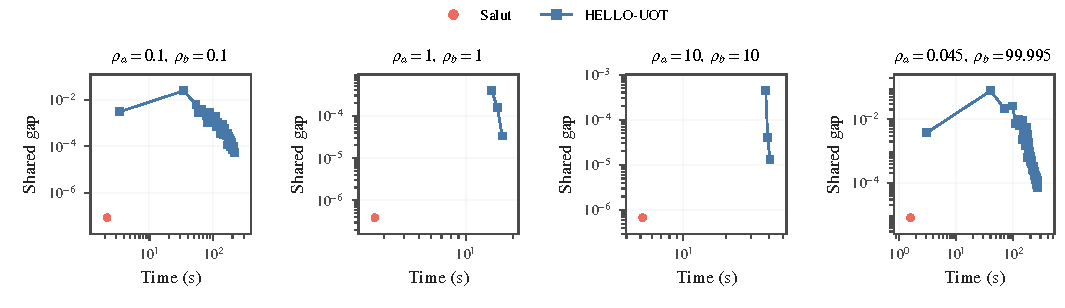
\includegraphics[width=\linewidth]{figures/hello_uot_gap_time_n32768.pdf}
\caption{$n=m=32{,}768$.}
\end{subfigure}
\par\smallskip
\begin{subfigure}{\linewidth}
\centering
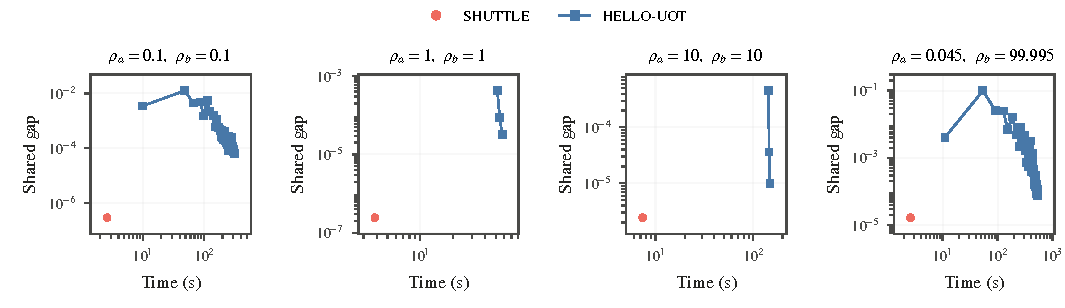
\includegraphics[width=\linewidth]{figures/hello_uot_gap_time_n65536.pdf}
\caption{$n=m=65{,}536$.}
\end{subfigure}
\par\smallskip
\begin{subfigure}{\linewidth}
\centering
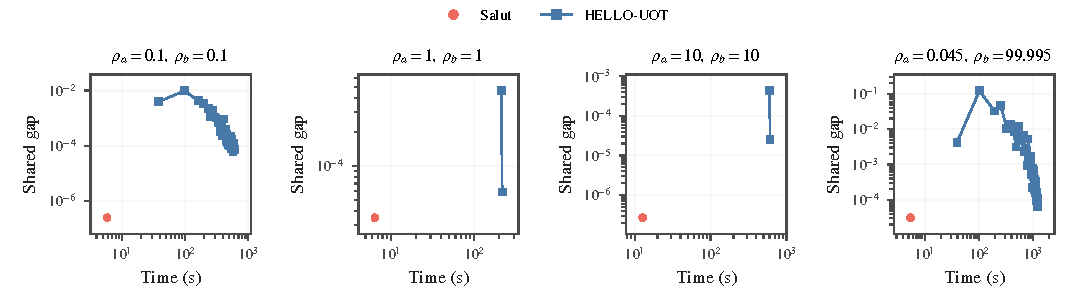
\includegraphics[width=\linewidth]{figures/hello_uot_gap_time_n131072.pdf}
\caption{$n=m=131{,}072$.}
\end{subfigure}
\caption{\textbf{\hellouot trajectories and final \ours solutions.}
Each row covers the four penalty pairs labeled above the panels on TOME E11.5$\to$E12.5 with $d=30$.
Blue squares trace observed \hellouot primal candidates after initialization and each outer oracle call; one coral point marks the final \ours solution at its complete solve time.
Both axes are logarithmic, and \sharedgap uses an independent audited lower bound for each instance.
Results use seed 42 with one run per method.}
\label{fig:hello-uot-trajectories}
\end{figure}
